\begin{tikzpicture}
	\node[circle, fill=Prune, text=white, draw=Prune] (n1) at (0,0){\ref*{chap:background}};
	\node[circle, fill=Prune, text=white, below=2.5cm of n1.south] (n2) {\ref*{chap:sota}};
	\node[circle, fill=Prune, text=white, below=2.5cm of n2.south] (n3) {\ref*{chap:attomics}};
	\node[circle, fill=Prune, text=white, below=2.5cm of n3.south] (n4) {\ref*{chap:crossattomics}};
	\node[circle, fill=Prune, text=white, below=2.5cm of n4.south] (n5){\ref*{chap:crossattomicsgate}};
	\node[circle, fill=Prune, text=white, below=2.5cm of n5.south] (n6){\ref*{chap:counterfactuals}};

	\draw[Prune, line width=3pt, dashed] (n1.north) -- +(0,1cm);
	\draw[Prune, line width=3pt] (n1.south) -- (n2.north);
	\draw[Prune, line width=3pt] (n2.south) -- (n3.north);
	\draw[Prune, line width=3pt] (n3.south) -- (n4.north);
	\draw[Prune, line width=3pt] (n4.south) -- (n5.north);
	\draw[Prune, line width=3pt] (n5.south) -- (n6.north);
	\draw[Prune, line width=3pt, -{Stealth}] (n6.south) -- +(0,-1cm);

	\tcbset{
		colframe=Prune,
		colback=white,
		colupper=Prune,
		fontupper=\footnotesize\hypersetup{linkcolor=Prune},
		fonttitle=\small\bfseries,
		nobeforeafter,
		tcbox width=auto limited,
		center title,
		width=6cm,
		left=1mm,right=1mm,top=1mm,bottom=1mm, boxsep=1.5mm
	}

	\node[right=1cm of n1.east, anchor=west] (b1) {
		\tcbox[title=Background]{
			In this chapter, I present the different deep learning architectures used during this thesis work and how to train them. A brief presentation of gene expression regulation and cancer formation is done. I also describe how the different omics are obtained. Finally, I describe the two datasets used: \glsxtrshort{tcga} and \glsxtrshort{ccle}.
		}
	};

	\node[left=1cm of n2.west, anchor=east] (b2) {
		\tcbox[title=State-of-the-art]{
			This chapter is dedicated to the description of the current deep learning methods used to predict a phenotype from omics data. I will also present multimodal deep learning and its application to integrate multi-omics data.
		}
	}; %4.85 cm available for images

	\node[right=1cm of n3.east, anchor=west] (b3) {
		\tcbox[title=AttOmics]{
			This chapter presents the AttOmics architecture, an architecture based on the attention mechanism. Expression profiles are transformed into groups of features with a transformation \(\symcal{T}\).
			Group are individually projected to compute intra-group interactions.
			\Glsxtrshort{mhsa} is then applied to incorporate inter-group interactions in the representation.
			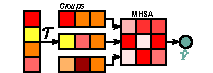
\includegraphics[width=\linewidth]{AttOmics_logo.pdf}
		}
	};

	\node[left=1cm of n4.west, anchor=east] (b4) {
		\tcbox[title=CrossAttOmics]{
			This chapter presents a multiomics extension of the AttOmics architecture. Each omics is encoded with an encoder based on AttOmics. Cross-attention is used to compute interactions between omics with known regulatory links.
			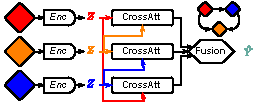
\includegraphics[width=\linewidth]{CrossAttOmics_Logo.pdf}
		}
	};

	\node[right=1cm of n5.east, anchor=west] (b5) {
		\tcbox[title=CrossAttOmicsGate]{
			This chapters present a variation of the CrossAttOmics architecture. Instead of focusing on known omics interactions, cross attention is used on all pairs of omics. Then interactions are scored for each patient.
			This importance score must have enough sparsity to be interpretable and diverse across samples, as omics interactions differ between samples.
		}
	};

	\node[left=1cm of n6.west, anchor=east] (b6) {
		\tcbox[title=Counterfactuals]{
			TEST tesfkl fzlkfes gznjef fe,fbzkf vjnfzefb
		}
	};

	\draw[Prune, line width=1.5pt, -{Circle}] (n1.east) -- (b1.west);
	\draw[Prune, line width=1.5pt, -{Circle}] (n2.west) -- (b2.east);
	\draw[Prune, line width=1.5pt, -{Circle}] (n3.east) -- (b3.west);
	\draw[Prune, line width=1.5pt, -{Circle}] (n4.west) -- (b4.east);
	\draw[Prune, line width=1.5pt, -{Circle}] (n5.east) -- (b5.west);
	\draw[Prune, line width=1.5pt, -{Circle}] (n6.west) -- (b6.east);

	\tcbhypernode{\hyperref[chap:background]}{n1}
	\tcbhypernode{\hyperref[chap:sota]}{n2}
	\tcbhypernode{\hyperref[chap:attomics]}{n3}
	\tcbhypernode{\hyperref[chap:crossattomics]}{n4}
	\tcbhypernode{\hyperref[chap:crossattomicsgate]}{n5}
	\tcbhypernode{\hyperref[chap:counterfactuals]}{n6}

	\tcbhypernode{\hyperref[chap:background]}{b1}
	\tcbhypernode{\hyperref[chap:sota]}{b2}
	\tcbhypernode{\hyperref[chap:attomics]}{b3}
	\tcbhypernode{\hyperref[chap:crossattomics]}{b4}
	\tcbhypernode{\hyperref[chap:crossattomicsgate]}{b5}
	\tcbhypernode{\hyperref[chap:counterfactuals]}{b6}
\end{tikzpicture}